\documentclass[a4paper]{article}

%% Language and font encodings
\usepackage[english]{babel}
\usepackage[utf8x]{inputenc}
\usepackage[T1]{fontenc}

%% Sets page size and margins
\usepackage[a4paper,top=3cm,bottom=2cm,left=3cm,right=3cm,marginparwidth=1.75cm]{geometry}

%% Useful packages
\usepackage{amsmath}
\usepackage{graphicx}
\usepackage{caption}
\usepackage{subcaption}
\usepackage[colorinlistoftodos]{todonotes}
\usepackage[colorlinks=true, allcolors=blue]{hyperref}

\title{Reporte de Actividad 10: Teoría del Caos y el Mapeo Logístico}
\author{Jesús Antonio González Espinosa \\ \\ Física Computacional 1}
\date{Miércoles, 16 de Mayo del 2018}

\begin{document}
\maketitle

\section{Introduction}
El mapeo logístico es un mapeo polinomial de segundo orden que ejemplifica como el comportamiento complejo y caótico puede surgir a partir de una ecuación dinámica no lineal muy simples. En esta actividad hemos de estudiarlo, y para eso, a partir de la bibliografía dada por la actividad que nos dirige al blog de Geoff Boeing, se va a hacer un resumen de sus resultados, tanto escritos como de sus gráficas que presenta. Como no se cuenta con el paquete que nos permite reproducir las gráficas en Python, nos vamos a apoyar de otra bibliografía de la actividad que nos ayuda a hacerlas en wxMaxima. A continuación, el resumen del blog de Boeing sobre el mapeo logístico.

\section{Resumen: Teoría del Caos y el Mapeo Logístico}
La teoría del caos es la rama de las matemáticas que trabaja con los sistemas dinámicos no lineales. Un sistema es un juego de componentes que interactuan que forman un todo; no lineales significa que por efectos multiplicativos entre los componentes, el entero se convierte en algo más grande que solo añadir las partes individuales; finalmente, dinámico significa que el sistema cambia con el tiempo en base a su estado actual. Los sistemas caóticos son un simple sub-tipo de sistemas dinámicos no lineales. Pueden contener pocas interacciones, pero mantienen una dependencia sensible en sus condiciones iniciales. Con el tiempo, estos sistemas pueden producir un comportamiento totalmente impredecible y divergente. Edward Lorenz describe el caos como "cuando el presente determina el futuro, pero el presente próximo no aproxima de forma determinada el futuro."

\subsection{EL Mapeo Logístico}
Vamos a explorar un ejemplo utilizando el famoso mapa logístico. Este modelo muestra una población que crece lento y luego rápido para finalmente disminuir, hasta llegar a su capacidad de carga. El mapeo logístico usa una ecuación de diferencia no lineal para ver los pasos del tiempo discretos. Se le llama así, porque mapea el valor de población en cualquier paso del tiempo a su valor al siguiente paso de tiempo:

\begin{center}
$x_(t+1) = rx_t(1-x_t)$
\end{center}

Esta ecuación define las reglas de nuestro sistema. $x$ representa la población en cualquier tiempo $t$, mientras que $r$ representa la tasa de crecimiento. Una tasa de crecimiento bajo lleva a la extinción, mientras que uno alto lleva a un boom de población.

Aquí, el autor con ayuda de python corre el modelo 20 veces con diferentes valores del parámetro de la tasa de crecimiento. Como esta tabla no se puede producir en wxMaxima.

\subsection{Comportamiento de Sistema y Atractores}
Un atractor es el juego de valores que el sistema establece con el tiempo. Cuando el parámetro de la tasa de crecimiento tiene un valor de 0.5,el sistema va a cero, con el tiempo; con un valor de 3.5 el sistema oscila entre cuatro valores. Este atractor es llamado ciclo límite. Cuando el valor del parámetro de la tasa de crecimiento va mayor a 3.5, se llega a un sistema caótico, con un atractor extraño, donde el sistema oscila por siempre; esto nos lleva a una estructura fractal, donde el mismo patrón se repite sin importar cuanto zoom se haga.

\begin{figure}[!ht]
 \centering
  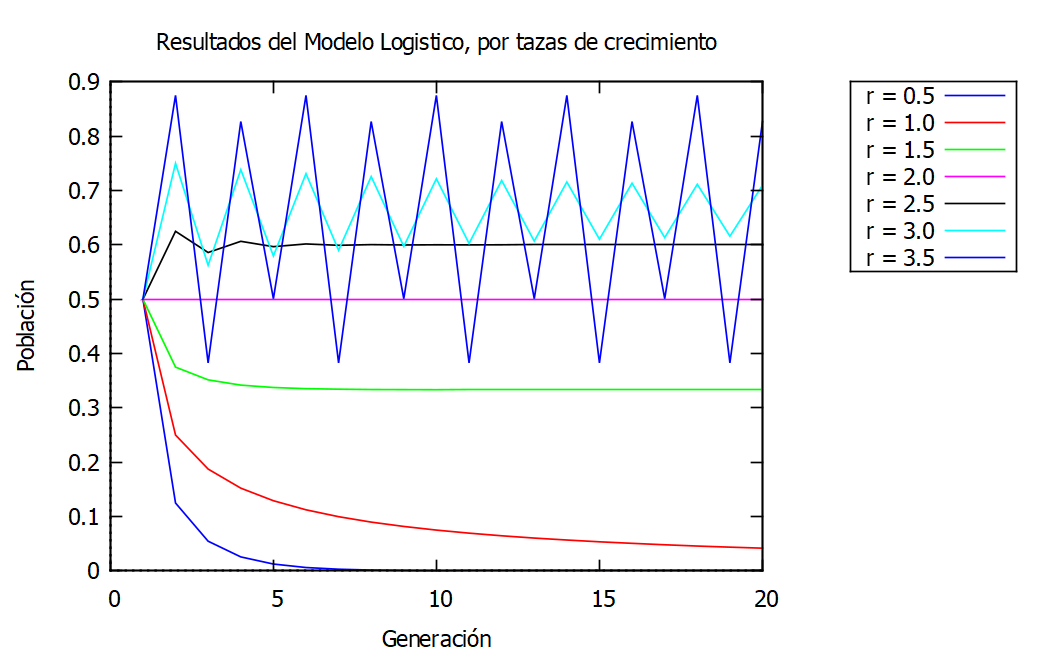
\includegraphics[width=0.75\textwidth]{GR05-35.png}
\end{figure}

En ésta, podemos ver como cambia la población con el tiempo, con diferentes tazas de crecimiento. Valores bajos, como 0.5, llevan a una población que rápidamente muere. Una taza de crecimiento con valor 2, muestra ser estable, mientras que 3 muestra llegar a una estabilidad después de un tiempo; finalmente 3.5 muestra muchos saltos de valores.
Un atractor es un valor o un conjunto de valores que cambian con el tiempo. Podemos ver que el atractor en 0.5 es 0, mientras que en 3.5 oscila entre cuatro valores. Esto se le conoce como ciclo límite. 
Al tener valores de tazas de crecimiento mayores a 3.5 llegamos a un sistema caótico, estos tienen atractores extraños en donde el sistema oscila por siempre. Estos muestran tener una estructura fractal.

\subsection{Bifurcación y el Camino al Caos}
Para mostrar esto, el autor corre el modelo de nuevo, esta vez con mil tasas de crecimiento entre 0.0 y 4.0 Para poder visualizar esto, hace un diagrama de bifurcación; al hacer esto en wxMaxima obtenemos:

\begin{figure}[!ht]
 \centering
  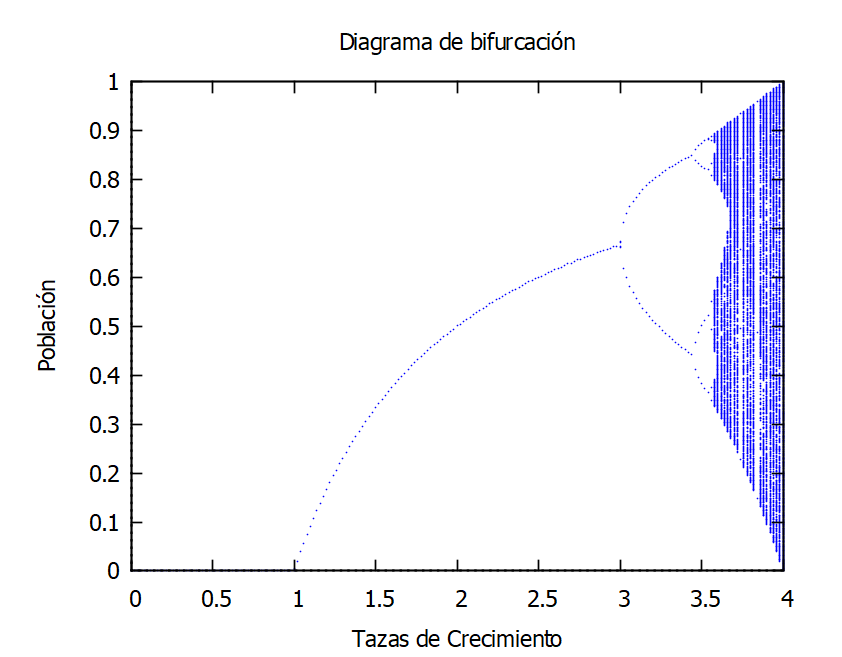
\includegraphics[width=0.75\textwidth]{Bifurcacion0-4.png}
\end{figure}

En cada corte vertical arriba de cada tasa de crecimiento es el atractor de ésta. 

Para crecimientos bajos como 1 o menos, vemos que el sistema colapsa a cero, para valores entre 1 y 3 podemos ver poblaciones estables y exactas. Pero al tener valores superiores, el diagrama muestra varios valores que no se ajustan a un punto o ciclo límite.


Al hacer zoom a los valores entre 2.8 y 4.0 obtenemos:

\begin{figure}[!ht]
 \centering
  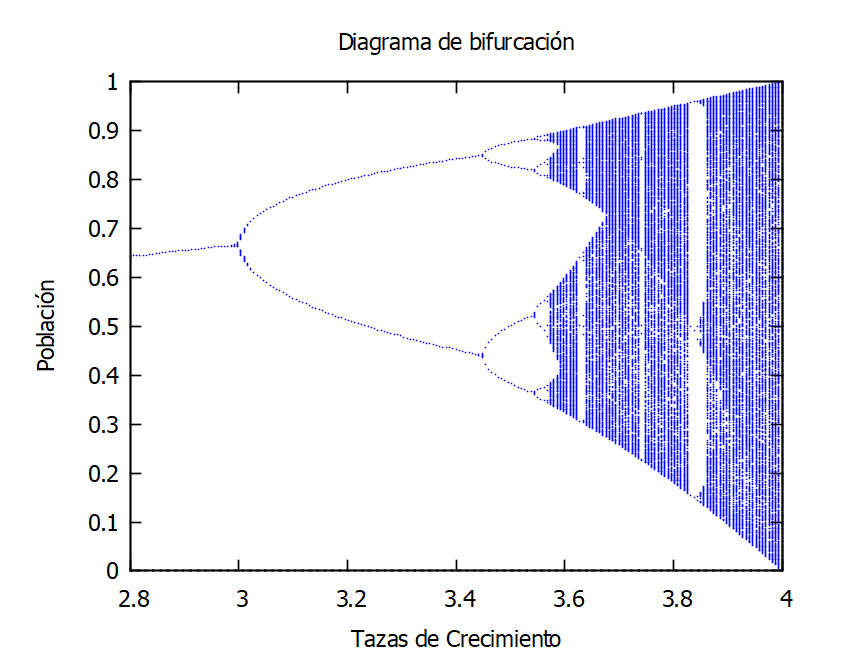
\includegraphics[width=0.75\textwidth]{Bifurcacion28-4.png}
\end{figure}

Podemos ver que a partir de ciertos valores de tazas de población, los valores se bifurcan, oscilando entre varios valores, cada vez separándose en más caminos.

\subsection{El Comienzo del Caos}

Podemos ver que a partir de ciertos valores en la tasa de crecimiento son capaces de tomar cualquier valor en la población. A esto se le conoce como el camino de periodo de duplicación al caos. El mapeo va a oscilar entre dos valores de población, luego cuatro, luego ocho y así continuamente. Estos son los periodos. Para cuando llegamos a la taza de crecimiento de 3.9, las bifurcaciones son tantas que parece que el sistema está aleatoria, aunque no es así, el modelo sigue reglas deterministas que parecen funcionar de forma aleatoria. Esto es el caos: determinista y aperiódico. Si hacemos zoom a las tasas de crecimiento entre 3.7 y 3.9 podemos ver:

\begin{figure}[!ht]
 \centering
  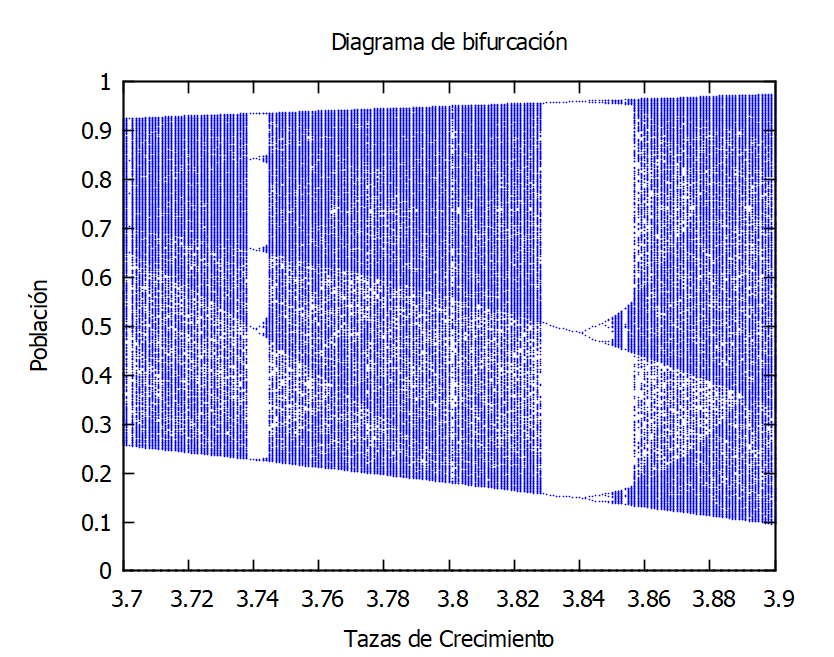
\includegraphics[width=0.65\textwidth]{Bifurcacion37-39.png}
\end{figure}

\pagebreak

Aquí podemos ver que entre el ruido se empieza a formar un patrón arremolinándose, específicamente entre tazas de crecimiento 3.82 y 3.84 podemos ver que el sistema va del caos al orden, oscilando entre tres valores de población, para luego volver a bifurcarse al caos.

\subsection{Fractales y Atractores Extraños}
En la gráfica anterior, podemos ver que la forma que toma en tazas de crecimiento de 3.85 es un poco familiar:

\begin{figure}[!ht]
 \centering
  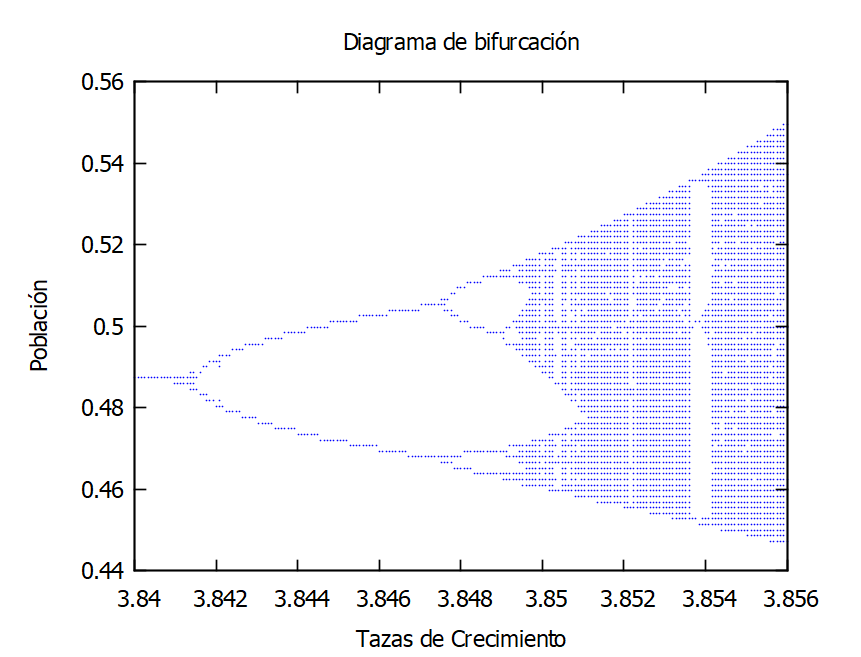
\includegraphics[width=0.8\textwidth]{Bifurcacion384-3856.png}
\end{figure}

Al hacer zoom entre los valores de 3.84 y 3.857, podemos observar la misma estructura que teníamos en el nivel macro. De hecho, si continuamos haciendo zoom, vamos a seguir viendo los mismos patrones. Como se mencionó antes, los sistemas caoticos tienen atractores extraños y que su estructura puede ser caracterizada como fractal. Los fractales tienen la misma estructura en cada escala; en esta escala podemos ver una reiteración de las mismas bifurcaciones, caos y ciclos limites que vimos en el diagrama de bifurcación completo. 

Otra manera de visualizar esto es con un diagrama de fase, que muestra el valor de población en una generación $t+1$ en el eje y, contra el valor de la población $t$ en el eje x. Hay que recordar que nuestro modelo sigue una simple regla determinista, por lo que si sabemos cierto valor de población de una generación, fácilmente podemos determinar el valor de la siguiente:

\begin{figure}[!ht]
\begin{subfigure}{0.6\textwidth}
  \centering
  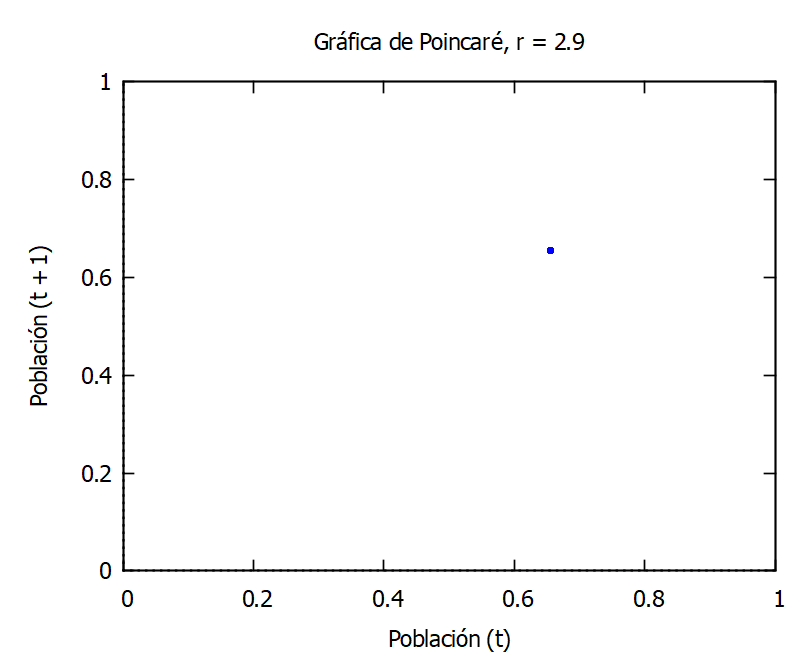
\includegraphics[width=0.8\linewidth]{Poincare29.png}
   \caption{r = 2.9}
\end{subfigure}
\begin{subfigure}{0.6\textwidth}
  \centering
  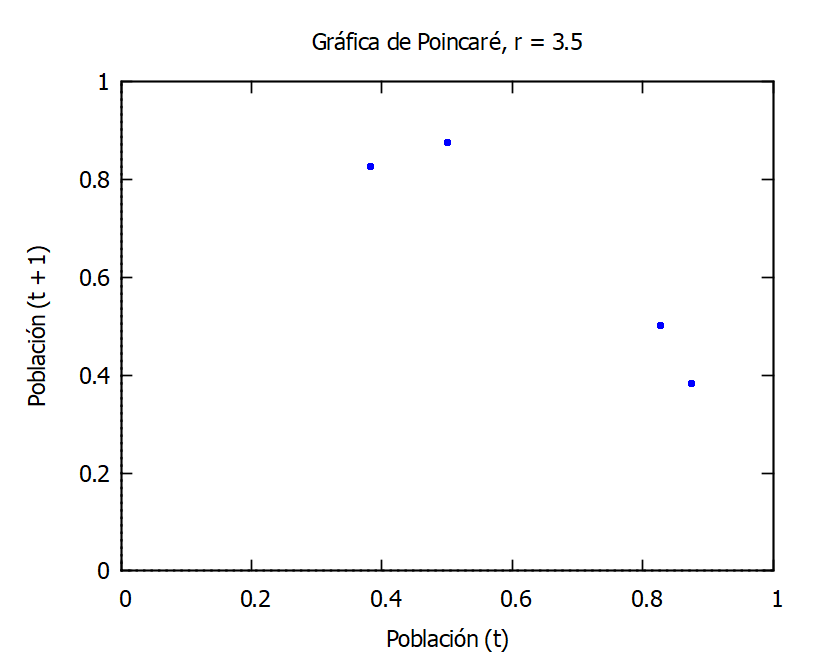
\includegraphics[width=0.8\linewidth]{Poincare35.png}
  \caption{r = 3.5}
\end{subfigure}
\end{figure}

\pagebreak

El diagrama de la izquierda muestra que cuando tenemos un parámetro de taza de crecimiento de 2.9, el mapeo logístico reside en un atractor de punto fijo en 0.655 en ambos ejes. En el diagrama de la derecha, muestra un atractor de ciclo límite, cuando la taza de crecimiento se fija en 3.5, el mapeo logístico oscila entre cuatro puntos. 

Esto es lo que sucede cuando estas bifurcaciones de periodo de duplicación llevan al caos:

\begin{figure}[ht!]
\begin{subfigure}{0.6\textwidth}
  \centering
  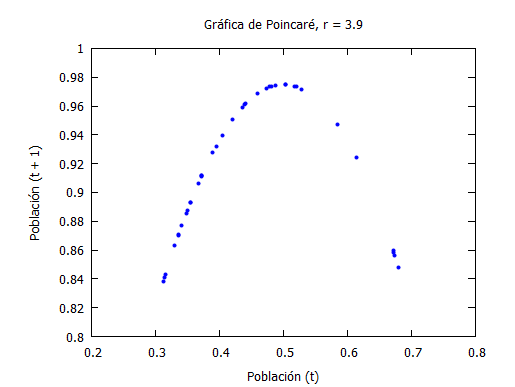
\includegraphics[width=0.8\linewidth]{Poincare39.png}
   \caption{r = 2.9}
\end{subfigure}
\begin{subfigure}{0.6\textwidth}
  \centering
  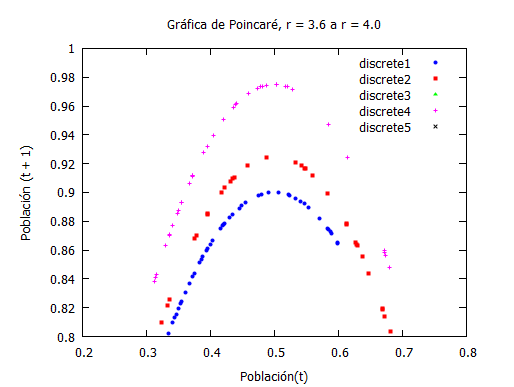
\includegraphics[width=0.8\linewidth]{Poincare36-4.png}
  \caption{3.6 < r < 4.0}
\end{subfigure}
\end{figure}

El rango de parámetros de las gráficas representan el régimen caótico: el rango de parámetros en donde el mapeo logístico se comporta de forma caótica. Cada taza de crecimiento forma su propia curva, donde ninguna se superposiciona una con otra por la geometría fractal y la naturaleza determinista de la ecuación logística. Los atractores extraños son revelados por estas figuras: el sistema está restringido, pero nunca se asienta a un punto fijo o una oscilación estable. 

\subsection{Caos contra Aleatoriedad}

Estos diagramas de fase muestran el estado de espacios 2-dimensional: un espacio imaginario que usa variables como sus dimensiones. Los diagramas de Fase son muy útiles para revelar atractores extraños, porque empotran estos datos 1-dimensionales dentro de estados de espacios 2 o 3-dimensionales. Ahora un ejemplo:

\begin{figure}[!ht]
 \centering
  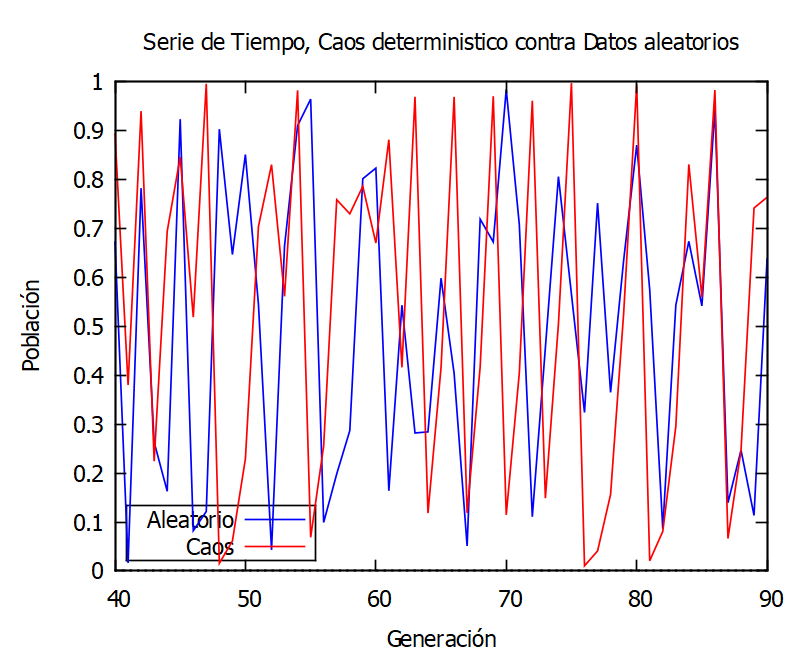
\includegraphics[width=0.8\textwidth]{Caos-Aleatorio.png}
\end{figure}

Una línea muestra saltos al azar, mientras que la otra no.

\begin{figure}[!ht]
 \centering
  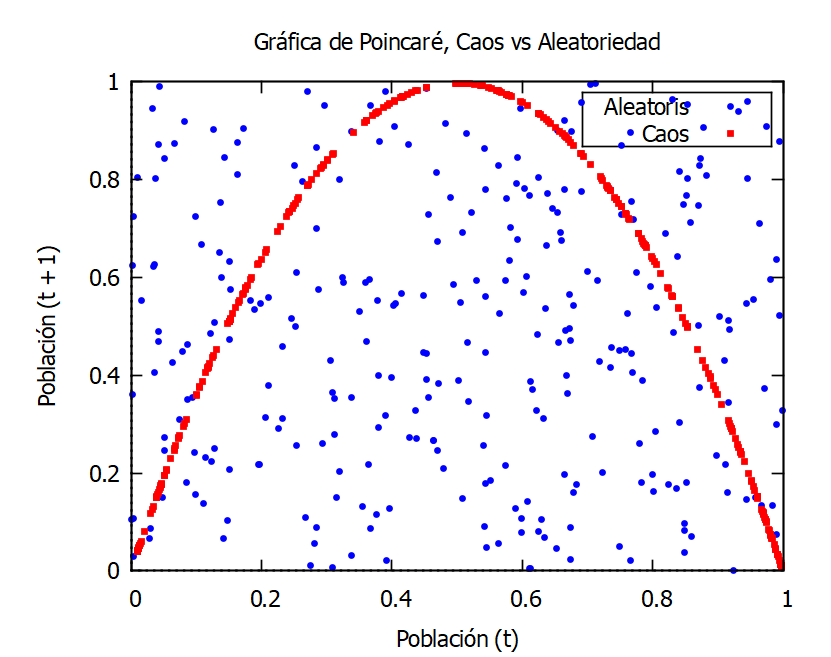
\includegraphics[width=0.8\textwidth]{Poincare-CaosAlea.png}
\end{figure}

Aqui vemos un sistema caotico (rojo) contenido por un atractor extraño contrastado con los datos al azar (azul).
En la tercera dimensión, podemos notar la estructura del a atractor extraño. 

\subsection{El Efecto Mariposa}
Los sistemas caoticos también son caracterizados por su sensibilidad a las condiciones iniciales; con un atractor extrapo, tienen puntos cercanos que divergen con el tiempo. Esto causa que la modelación y predición de la vida real sea difícil, requiriendo una infinidad de precisión en las medidas; de lo contrario, los errores con el tiempo van a irse acumulando, arruinando el sistema. Así es como Lorenz, a partir de un error de redondeo, descubrió el caos. 

\begin{figure}[!ht]
 \centering
  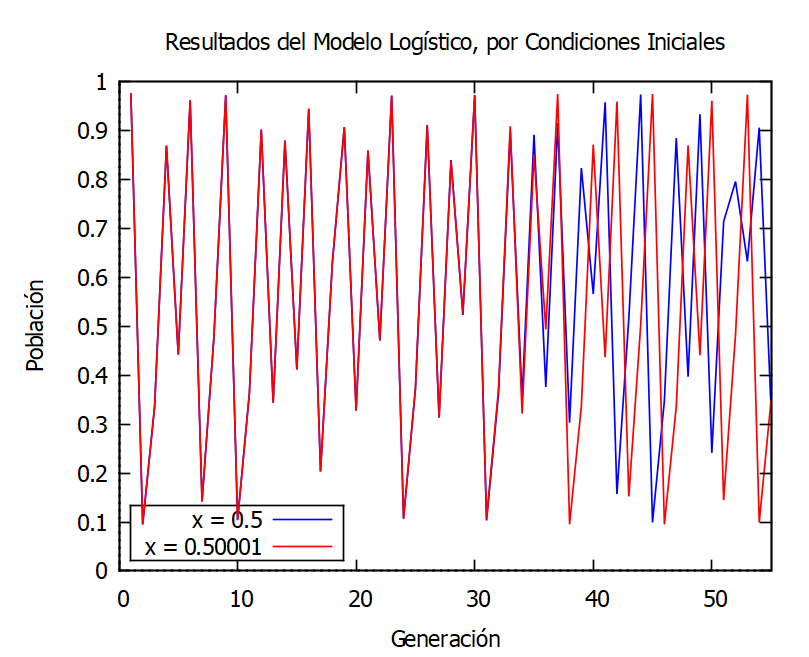
\includegraphics[width=0.8\textwidth]{GR05050001.png}
\end{figure}

En la gráfica podemos ver como hay dos líneas con una población inicial muy parecida y con un parámetro en la taza de crecimiento de 3.9; podemos notar como en el inicio son muy parecidos, pero después de ciertas generaciones, se van alejando, hasta ya no tener ningún parecido. Con el caos, la historia está perdida en el tiempo y las predicciones del futuro solo son tan precisas como nuestras medidas. En los sistemas caóticos del mundo real, las medidas nunca son totalmente precisas, por lo que el futuro se vuelve impredecible a partir de cierto punto.

Esto es conocido como el efecto mariposa: una aleteada de la ala de una mariposa en China puede causar un tornado en Texas. Pequeños eventos se acumulan e irreversiblemente afectan el futuro. 

\subsection{Las Implicaciones del Caos}
Se presentan ejemplos de sistemas caóticos y fractales en el mundo real incluyendo 
fugas, helechos, frecuencia cardíaca y generadores de números aleatorios. El caos, fundamentalmente indica que hay límites para el conocimiento y la predicción. 

\section{Conclusión}
En esta actividad vimos el verdadero potencial que tiene wxMaxima, ya que en la pasada fue una simple exploración teórica; ahora trabajamos de primera mano con él, para explorar el Mapeo Logístico. Fue una actividad muy interesante, ya que se complico mucho el trabajo; de todas, en lo personal creo que esta ha sido la que ha presentado el más grande reto. Fue mucha la investigación necesaria, en tanto los manuales en línea como en el que se hizo en la actividad pasada. Además de que el proceso de graficación resulto algo tedioso, pero una vez que ya se entendía el concepto del proceso, la actividad pudo ser efectuada sin más trabas. 



\section{Bibliografía}
\begin{enumerate}
\item Boeing, G. (2015) Chaos Theory and Logistic Map. Recuperado el 16 de Mayo del 2018 desde http://geoffboeing.com/2015/03/chaos-theory-logistic-map/
\item Morante, A., Vallejo, J. (2013) Chaotic dynamics with Maxima. Recuperado el 16 de Mayo del 2018 desde https://arxiv.org/pdf/1301.3240.pdf
\end{enumerate}

                         
\end{document}